\documentclass[tikz,border=5pt,multi=tikzpicture]{standalone}
\usepackage{amsmath}
\usepackage{pgfplots}
\pgfplotsset{compat=1.18}
\usetikzlibrary{calc,intersections}

\definecolor{epcgreen}{HTML}{1F684F}
\definecolor{epcblue}{HTML}{2D6F9F}
\definecolor{epcgold}{HTML}{BD7A1E}
\definecolor{epcred}{HTML}{BF4D42}
\definecolor{epcink}{HTML}{172026}
\definecolor{epcgrid}{HTML}{DDE7E3}

\pgfplotsset{
  epcaxis/.style={
    width=9cm,
    height=6cm,
    axis lines=left,
    xmin=0,
    ymin=0,
    grid=both,
    major grid style={draw=epcgrid, line width=0.35pt},
    minor grid style={draw=epcgrid!60, line width=0.2pt},
    minor tick num=1,
    tick style={draw=none},
    ticklabel style={font=\scriptsize, color=epcink},
    label style={font=\small, color=epcink},
    legend style={
      draw=none,
      fill=white,
      font=\scriptsize,
      cells={anchor=west}
    },
    clip=false
  },
  epcline/.style={smooth, line width=1.2pt},
  guide/.style={dashed, draw=epcink!35, line width=0.45pt},
  point/.style={only marks, mark=*, mark size=2.2pt, draw=white, line width=0.5pt}
}

\tikzset{
  guide/.style={dashed, draw=epcink!35, line width=0.45pt}
}

\begin{document}

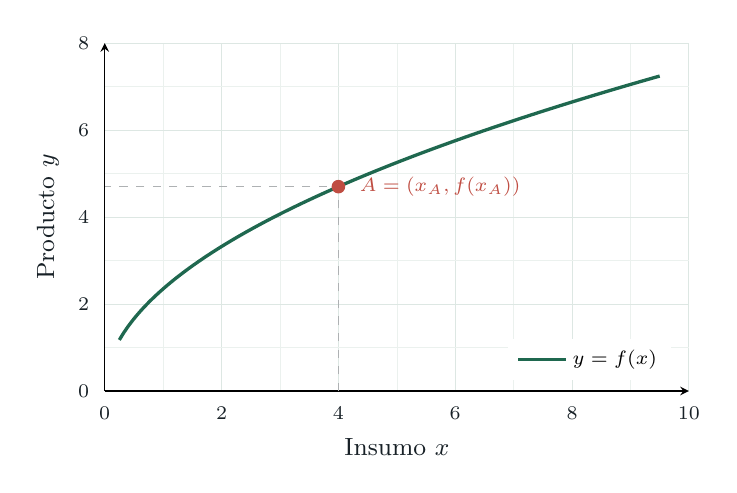
\begin{tikzpicture}
  \begin{axis}[
    epcaxis,
    xmax=10,
    ymax=8,
    xlabel={Insumo $x$},
    ylabel={Producto $y$},
    legend pos=south east
  ]
    \addplot[epcline, color=epcgreen, domain=0.25:9.5, samples=120] {2.35*sqrt(x)};
    \addlegendentry{$y=f(x)$}
    \addplot[point, color=epcred] coordinates {(4,4.7)};
    \draw[guide] (axis cs:4,0) -- (axis cs:4,4.7) -- (axis cs:0,4.7);
    \node[font=\scriptsize, color=epcred, anchor=west] at (axis cs:4.2,4.7) {$A=(x_A,f(x_A))$};
  \end{axis}
\end{tikzpicture}

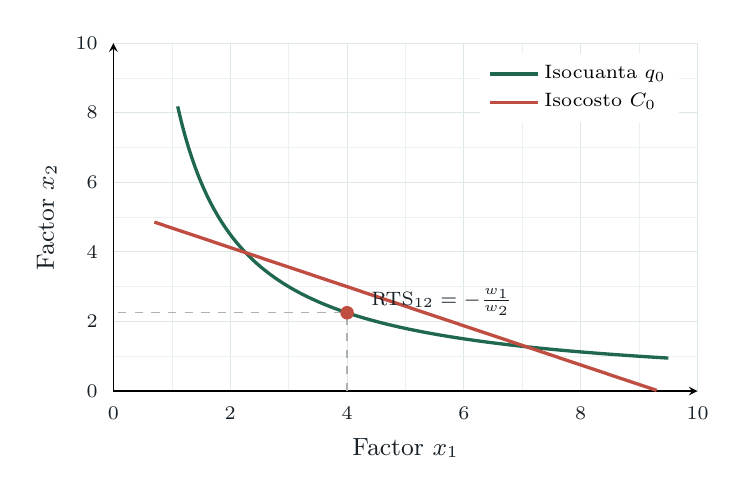
\begin{tikzpicture}
  \begin{axis}[
    epcaxis,
    xmax=10,
    ymax=10,
    xlabel={Factor $x_1$},
    ylabel={Factor $x_2$},
    legend pos=north east
  ]
    \addplot[epcline, color=epcgreen, domain=1.1:9.5, samples=140] {9/x};
    \addlegendentry{Isocuanta $q_0$}
    \addplot[epcline, color=epcred, domain=0.7:9.3, samples=2] {-0.5625*x+5.25};
    \addlegendentry{Isocosto $C_0$}
    \addplot[point, color=epcred] coordinates {(4,2.25)};
    \draw[guide] (axis cs:4,0) -- (axis cs:4,2.25) -- (axis cs:0,2.25);
    \node[font=\scriptsize, color=epcink, anchor=west] at (axis cs:4.25,2.55) {$\operatorname{RTS}_{12}=-\frac{w_1}{w_2}$};
  \end{axis}
\end{tikzpicture}

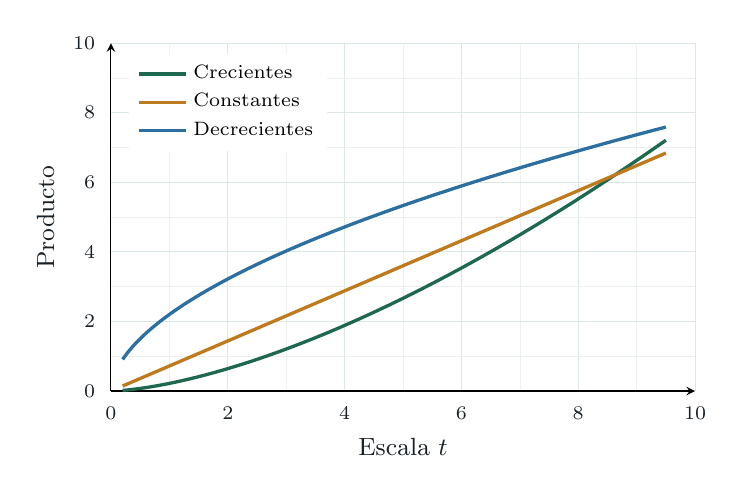
\begin{tikzpicture}
  \begin{axis}[
    epcaxis,
    xmax=10,
    ymax=10,
    xlabel={Escala $t$},
    ylabel={Producto},
    legend pos=north west
  ]
    \addplot[epcline, color=epcgreen, domain=0.2:9.5, samples=120] {0.22*x^1.55};
    \addlegendentry{Crecientes}
    \addplot[epcline, color=epcgold, domain=0.2:9.5, samples=2] {0.72*x};
    \addlegendentry{Constantes}
    \addplot[epcline, color=epcblue, domain=0.2:9.5, samples=120] {2.2*x^0.55};
    \addlegendentry{Decrecientes}
  \end{axis}
\end{tikzpicture}

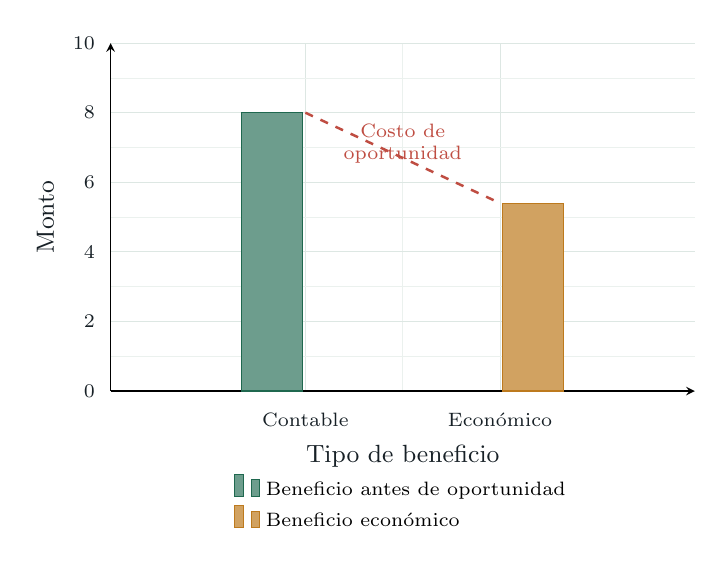
\begin{tikzpicture}
  \begin{axis}[
    epcaxis,
    ybar,
    bar width=22pt,
    xmax=3,
    ymax=10,
    xmin=0,
    xtick={1,2},
    xticklabels={Contable,Económico},
    ylabel={Monto},
    xlabel={Tipo de beneficio},
    legend style={at={(0.5,-0.22)}, anchor=north, legend columns=1}
  ]
    \addplot[fill=epcgreen!65, draw=epcgreen] coordinates {(1,8)};
    \addlegendentry{Beneficio antes de oportunidad}
    \addplot[fill=epcgold!70, draw=epcgold] coordinates {(2,5.4)};
    \addlegendentry{Beneficio económico}
    \draw[epcred, line width=0.9pt, dashed] (axis cs:1,8) -- (axis cs:2,5.4);
    \node[font=\scriptsize, color=epcred, align=center] at (axis cs:1.5,7.1) {Costo de\\oportunidad};
  \end{axis}
\end{tikzpicture}

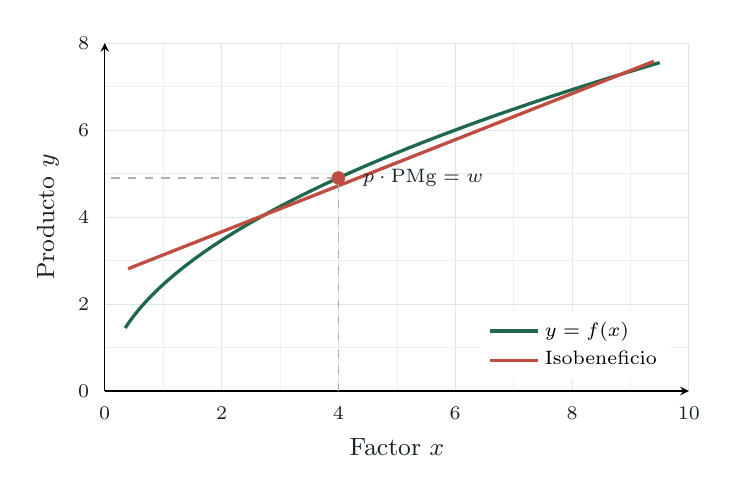
\begin{tikzpicture}
  \begin{axis}[
    epcaxis,
    xmax=10,
    ymax=8,
    xlabel={Factor $x$},
    ylabel={Producto $y$},
    legend pos=south east
  ]
    \addplot[epcline, color=epcgreen, domain=0.35:9.5, samples=120] {2.45*sqrt(x)};
    \addlegendentry{$y=f(x)$}
    \addplot[epcline, color=epcred, domain=0.4:9.4, samples=2] {0.53*x+2.6};
    \addlegendentry{Isobeneficio}
    \addplot[point, color=epcred] coordinates {(4,4.9)};
    \draw[guide] (axis cs:4,0) -- (axis cs:4,4.9) -- (axis cs:0,4.9);
    \node[font=\scriptsize, color=epcink, anchor=west] at (axis cs:4.25,4.9) {$p\cdot \operatorname{PMg}=w$};
  \end{axis}
\end{tikzpicture}

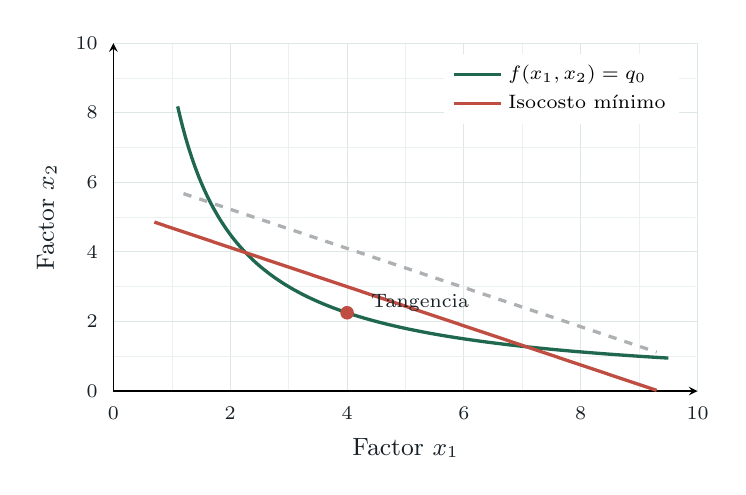
\begin{tikzpicture}
  \begin{axis}[
    epcaxis,
    xmax=10,
    ymax=10,
    xlabel={Factor $x_1$},
    ylabel={Factor $x_2$},
    legend pos=north east
  ]
    \addplot[epcline, color=epcgreen, domain=1.1:9.5, samples=140] {9/x};
    \addlegendentry{$f(x_1,x_2)=q_0$}
    \addplot[epcline, color=epcred, domain=0.7:9.3, samples=2] {-0.5625*x+5.25};
    \addlegendentry{Isocosto mínimo}
    \addplot[epcline, color=epcink!35, dashed, domain=1.2:9.3, samples=2] {-0.5625*x+6.35};
    \addplot[point, color=epcred] coordinates {(4,2.25)};
    \node[font=\scriptsize, color=epcink, anchor=west] at (axis cs:4.25,2.55) {Tangencia};
  \end{axis}
\end{tikzpicture}

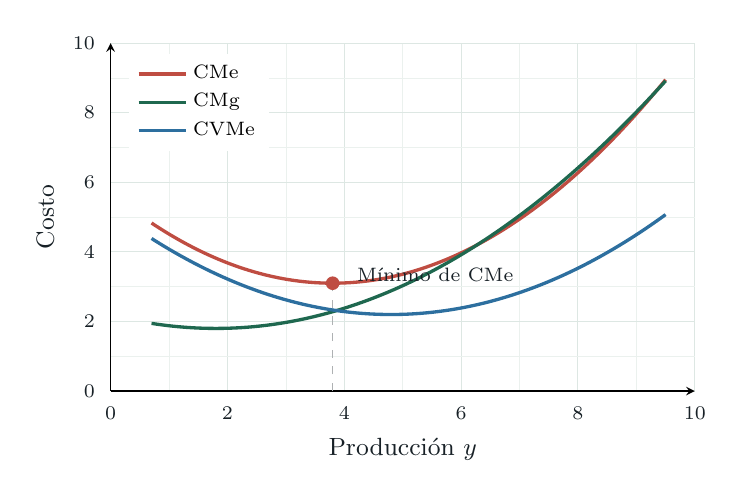
\begin{tikzpicture}
  \begin{axis}[
    epcaxis,
    xmax=10,
    ymax=10,
    xlabel={Producción $y$},
    ylabel={Costo},
    legend pos=north west
  ]
    \addplot[epcline, color=epcred, domain=0.7:9.5, samples=140] {0.18*(x-3.8)^2+3.1};
    \addlegendentry{$\operatorname{CMe}$}
    \addplot[epcline, color=epcgreen, domain=0.7:9.5, samples=140] {0.12*(x-1.8)^2+1.8};
    \addlegendentry{$\operatorname{CMg}$}
    \addplot[epcline, color=epcblue, domain=0.7:9.5, samples=140] {0.13*(x-4.8)^2+2.2};
    \addlegendentry{$\operatorname{CVMe}$}
    \addplot[point, color=epcred] coordinates {(3.8,3.1)};
    \draw[guide] (axis cs:3.8,0) -- (axis cs:3.8,3.1);
    \node[font=\scriptsize, color=epcink, anchor=west] at (axis cs:4.05,3.35) {Mínimo de $\operatorname{CMe}$};
  \end{axis}
\end{tikzpicture}

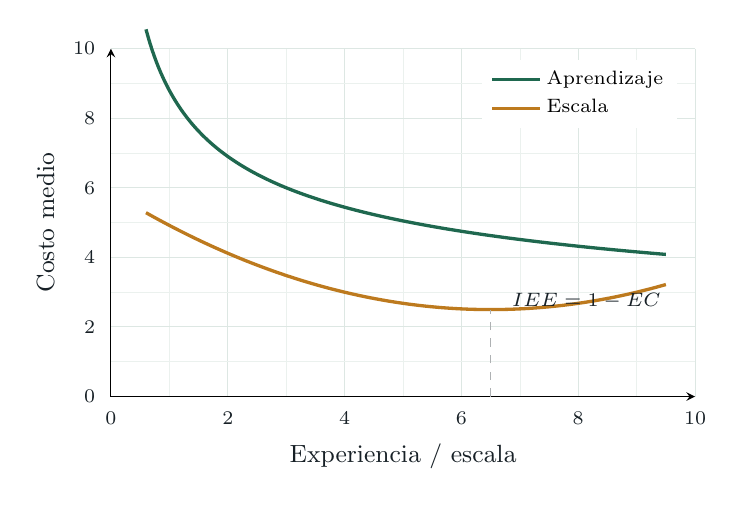
\begin{tikzpicture}
  \begin{axis}[
    epcaxis,
    xmax=10,
    ymax=10,
    xlabel={Experiencia / escala},
    ylabel={Costo medio},
    legend pos=north east
  ]
    \addplot[epcline, color=epcgreen, domain=0.6:9.5, samples=140] {8.2/(x^0.38)+0.6};
    \addlegendentry{Aprendizaje}
    \addplot[epcline, color=epcgold, domain=0.6:9.5, samples=140] {0.08*(x-6.5)^2+2.5};
    \addlegendentry{Escala}
    \draw[guide] (axis cs:6.5,0) -- (axis cs:6.5,2.5);
    \node[font=\scriptsize, color=epcink, anchor=west] at (axis cs:6.7,2.75) {$IEE=1-EC$};
  \end{axis}
\end{tikzpicture}

\end{document}
